\begin{subappendices}
\section{Inference Rules}
\label{sec:appendix:inference-rules}
In Figure~\ref{fig:inference}, we provide the rules used to determining the constraints and guarantees for a specification.
We represent $ 
X \odot Y : (E, \epsilon, \delta) \equiv \Pr\left(| \E[X] \odot \E[Y] - E | \geq \epsilon \right) \leq \delta
$
where $\odot$ represents a binary operator.
Constraints are represented in $\{ \}$.
%\pmcomment{Need to explain that constraints carry over in missing cases in Figure!\ref{fig:inference}}
%\pmcomment{Add proofs here for inference rules.}
The proof of correctness for each inference rule starts from the assumptions above the horizontal line and derives the assertions below. 
These proofs use ideas similar to those in \cite{bastani2019probabilistic}.
We reproduce the proofs in Appendix~\ref{sec:appendix:constraint:proofs} here for completeness.
%We provide them here for completeness.
Note that the assertions in the base case (elementary subexpressions) can be arrived at by applying $\rm{AIN}$. 

\begin{figure}
\[
\dfrac{X: \left(\BarE[X], \epsilon_X, \delta_X\right), Y: \left(\BarE[Y], \epsilon_Y, \delta_Y\right)}{X \pm Y: \left(\BarE[X] \pm \BarE[Y], \epsilon_X + \epsilon_Y, \delta_X + \delta_Y\right)}
\]
\[
\dfrac{X: \left(\BarE[X], \epsilon_X, \delta_X\right), Y: \left(\BarE[Y], \epsilon_Y, \delta_Y\right)}{ X \times Y: (\BarE[X] \BarE[Y], \epsilon_X \epsilon_Y + \BarE[X] \epsilon_Y + \BarE[Y] \epsilon_X, \delta_X + \delta_Y)} 
\]
\[
\dfrac{X: \left(\BarE, \epsilon, \delta \right), \BarE - \epsilon > 0}{ X^{-1}: \left(\BarE^{-1}, \frac{\epsilon}{\BarE (\BarE - \epsilon)}  , \delta \right)}\text{ (Inverse)} 
\] 
\[
\dfrac{X: \left(\BarE, \epsilon, \delta \right)}{ X^{-1}: \left(\BarE^{-1}, \frac{\epsilon}{\BarE (\BarE - \epsilon)}  , \delta \right), \{ \BarE - \epsilon > 0\}} \text{ (Inverse C)}
\]
\[
\dfrac{X: \left(\BarE, \epsilon, \delta\right), \BarE - \epsilon > c}{ X > c: (T, \delta)} \text{ (True)} \hspace{0.1in} \dfrac{X: \left(\BarE, \epsilon, \delta \right), \BarE  + \epsilon < c}{ X < c: (F, \delta)} \text{ (False)} 
\] 
\[
\dfrac{X: \left(\BarE, \epsilon, \delta\right)}{ X > c: (T, \delta), \{\BarE - \epsilon > c\}} \text{ (True C)} \]
\[
\dfrac{X: \left(\BarE, \epsilon, \delta \right)}{ X < c: (T, \delta), \{\BarE + \epsilon < c\}} \text{ (False C)} 
\] 
\[
\dfrac{\psi_1: (\B_1, \delta_1), \psi_2: (\B_2, \delta_2)}{\psi_1 \wedge \psi_2: (\B_1 \wedge \B_2, \delta_1 + \delta_2)} \text{ (and)} \hspace{0.01in} \dfrac{\psi_1: (\B_1, \delta_1), \psi_2: (\B_2, \delta_2)}{\psi_1 \vee \psi_2: (\B_1 \vee \B_2, \delta_1 + \delta_2)} \text{ (or)}
\]
\[
\dfrac{\psi_1: (\B_1, \delta_1), \{C_{11, \dots, 1k}\}, \psi_2: (\B_2, \delta_2), \{C_{21, \dots, 2m}\}}{\psi_1 \wedge \psi_2: (\B_1 \wedge \B_2, \delta_1 + \delta_2), \{C_{11, \dots, 1k}, C_{21, \dots, 2m}\}} \text{ (and C)} \]
\[
\hspace{0.2in} \dfrac{\psi_1: (\B_1, \delta_1), \{C_{11, \dots, 1k}\}, \psi_2: (\B_2, \delta_2)}{\psi_1 \vee \psi_2: (\B_1 \vee \B_2, \delta_1 + \delta_2),  \{C_{11, \dots, 1k}\} \vee \{C_{21, \dots, 2m}\}} \text{ (or C)}
\]%
\caption{Inference rules used to guarantees for expressions.The inference rules for each compound expression build on the union bound, triangle inequality, and structural induction approach described by \citet{bastani2019probabilistic}. C: Constraint.}
\label{fig:inference}
\end{figure}
\subsection{Inference rules with Constraints}
\label{sec:appendix:constraint:proofs}

%We define guarantees for concentration using an appropriate concentration inequality. 
%Examples are provided in the Appendix~\ref{sec:appendix:inequality}  
%\paragraph{Correctness} 
In Section~\ref{sec:theoretical:propagation} we provided the proofs for $X\pm Y$, $X > c$.
In the following text, we provide the remaining proofs.

\noindent \textit{Product} Starting with $\phi_X, \phi_Y$
%$\phi_X \eqdef (\BarE[X], \epsilon_X, \delta_X)$, $\phi_Y = Y: (\BarE[Y], \epsilon_Y, \delta_Y)$. 
First, from union bound, both of these hold true with probability at least $1 - \delta_X - \delta_Y$.
Then,
{\allowdisplaybreaks
\begin{align*}
|\E[X]| &= |\BarE[X] - \BarE[X] + \E[X]|\\
        &\leq ||\BarE[X]| +  |\BarE[X] + \E[X]| \leq ||\BarE[X]| + \epsilon_X \\
\end{align*}
}
%We have
\begin{align*}
    |\BarE[X]\BarE[Y] &- \E[XY]|  = |\BarE[X]\BarE[Y]  - \E[X]\E[Y]| \\
    %&= |\BarE[X]\BarE[Y] - \BarE[X]\E[Y] + \BarE[X]\E[Y]  - \E[X]\E[Y]| \\
    &= |\BarE[X](\BarE[Y] - \E[Y]) + \E[Y] (\BarE[X]\  - \E[X])| \\
    &\leq |\BarE[X]||(\BarE[Y] - \E[Y])| + |\E[Y]||(\BarE[X]\  - \E[X])| \\
    &\leq |\BarE[X]| \eps_Y + |\E[Y]| \eps_X \\
    &\leq |\BarE[X]| \eps_Y + (|\BarE[Y]| + \eps_Y) \eps_X \\
    &= |\BarE[X]| \eps_Y + |\BarE[Y]| \eps_X + \eps_X \eps_Y
\end{align*}
where the first step follows as $X, Y$ are Bernoulli r.vs.
Therefore, $X \times Y: (\BarE[X] \BarE[Y], \epsilon_X \epsilon_Y + \BarE[X] \epsilon_Y + \BarE[Y] \epsilon_X, \delta_X + \delta_Y)$

\textit{Inverse/Inverse C} Assume $X: \left(\BarE, \epsilon, \delta \right)$ and $\BarE - \epsilon > 0$.
In the constrained case, we start with only the prior assumption. % i.e., $X: \left(\BarE, \epsilon, \delta \right)$
Then,
\begin{align*}
    |\E[X]| &= |\E[X] - \BarE[X] + \BarE[X]| \\
    &\leq |\E[X] - \BarE[X]| + |\BarE[X]| \leq \epsilon_X + |\BarE[X]|
\end{align*}
i.e., $|\E[X]| \leq \epsilon_X + |\BarE[X]|$. 
Also,
\begin{align*}
    |\E[X]^{-1} - \BarE[X]^{-1}| &= \left|\frac{\BarE[X]^{-1} - \E[X]^{-1}}{\BarE[X]  \E[X]^{-1}}\right| \\
    &\leq \frac{\epsilon}{|\E[X]|  |\BarE[X]|} \leq \frac{\epsilon}{|\E[X]| (\E[X] - \epsilon_X)}
\end{align*}
%where the last step follows from the previous derivation and if $\E[X] - \epsilon_X > 0$.
%The latter condition enforces that the sign of the inequality does not change.
VF adds $E[X] - \epsilon_X > 0$ as a precondition; \AVOIRmethodname{} as a post-constraint.
\paragraph{Boolean Operators}
Starting from $\psi_1: (b_1, \delta_1)$, $\psi_2: (b_2, \delta_2)$, we can apply the union bound for $\psi_1 \wedge \psi_2$, $\psi_1 \vee \psi_2$ to derive the rules for and/or.
%\pmcomment{TODO: Complete Proofs}
Similarly, constraints follow the semantics specified by the rules as they also follow from the union bound.




\subsection{Inferred Optimization Problem}
\label{sec:appendix:inferrence-rules:opt}
For a given overall specification $\psi$, suppose $(\epsilon_i, \delta_i$), $i \in \{1, \dots, n\}$ represents the concentration bounds associated with each constituent elementary subexpression. 
Using the inference rules, we can derive the overall $\delta_T = \sum\limits_{i}\delta_i$, along with a set of (say) $K$ constraints 
\[
g_k(\epsilon_{1}, \dots, \epsilon_{n}, \BarE[X_1], \dots, \BarE[X_n]) \leq \epsilon_k
\]
\[
\text{where } \epsilon_k = \left|c_k - \BarE[f(\BarE[X_1], \dots, \BarE[X_n])]\right|
\]
denotes the maximum allowed margin for the $\text{k}^{\text{th}}$ subexpression of form \texttt{<ETerm> <comp-op> c}).
The objective is to minimize the overall failure probability $\delta_T$.
The overall optimization problem can then be formulated as shown in \ref{eq:optimization},
having $n$ optimization variables $\delta_i$ and $2n + K$ constraints (bounds on $\delta_i$ provide the $2n$ constraints).  
A developer using \AVOIRmethodname{} inputs a required acceptable upper bound of failure probability $\Delta$.
If the solution to the optimization problem $\delta_T^* = \sum_i \delta_i \leq \Delta$, then the optimization can conclude with the required confidence in the proved guarantee.
At this point, the developer may choose to terminate \AVOIRmethodname{}.
However, using Corollary~\ref{thm:adaptive-stopping:anytime}, they may continue to run and refine the estimates.

% Metrics table


\section{Concentration bounds}
%Recall the adaptive Hoeffding inequality~\citep{zhao2016adaptive, bastani2019probabilistic} from \Cref{thm:adaptive-stopping}. 

%\AIN*
%\newtheorem{theorem}{Theorem} % TODO: move to my_definitions.tex


Theorem~\ref{thm:adaptive-stopping} provides a mechanism for choosing the stopping time using arbitrary methods for a fixed $\delta$. 
In general, any adaptive concentration inequality suffices; we use $\rm{AIN}_H$ %that does not depend on the empirical variance but is frequently used in scenarios dealing with bounded r.vs.
However, we use confidence intervals to visualize the evolution of sub-expressions (and overall specification) over the sequence of observations. 
To do so, we require an additional result.

\begin{theorem}\cite[Proposition 1, Lemma 1]{zhao2016adaptive}
Let $S_n = \sum_{i=1}^n X_i$ be a random walk from i.i.d. random variables $X_1, \dots, X_t \sim D$. For any $\delta > 0$,
$\Pr[S_\gT \geq f(\gT)] \leq \delta$
for any stopping time $\gT$ if and only if
$\Pr\left[\exists n, S_t \geq f(t) \right] \leq \delta$

\label{thm:zhao:adaptive-hoeffding:anytime}
\end{theorem}

\begin{corollary}
\label{thm:adaptive-stopping:anytime}
For $\delta > 0$, $\Pr[|\BarE_\gT[X] - \E[X]| \leq \epsilon(\delta, \gT)|] \geq 1 - \delta $
for any stopping time $\gT$ if and only if
\[
\Pr\left[\forall t, |\BarE_t[X] - \E[X]| \leq \epsilon(\delta, t)| \right] \geq 1 - \delta
\]
\end{corollary}
%\begin{proof}
%\pmcomment{need to correct this} 
Corollary~\ref{thm:zhao:adaptive-hoeffding:anytime} follows directly from applying Theorem~\ref{thm:zhao:adaptive-hoeffding:anytime} to Theorem~\ref{thm:adaptive-stopping}.
%\end{proof}
Intuitively, Theorem~\ref{thm:adaptive-stopping} holds since we can choose an adversarial stopping rule for $\gT$ that terminates as soon as the boundary for $\epsilon(\delta, t)$ is crossed~\citep{zhao2016adaptive}. 
Thus, when we establish a bound with a stopping rule, %, as long as the underlying distribution remains unchanged,
the bound will hold prior to and after the stopping rule is enforced.
Corollary~\ref{thm:adaptive-stopping:anytime} implies that once we choose an optimal bound for each subexpression, we can extend the bounds derived using Theorem~\ref{thm:adaptive-stopping} to following observations with continued guarantees for subexpressions.
%Note that this does not necessarily imply that the specification will still be True/False with a bounded failure probability since the truth value of the specification depends on the empirical mean.

\subsection{Proof of Theorem~\ref{thm:conf-seq} for Specifications}
\label{sec:thm:conf-seq:proof:contd}

%Recall \Cref{thm:conf-seq}
%\confseq*

Consider any specification $\psi_k$. Let $\psi_k^t : (\hat{b}_{\psi_k}(t), \delta_{\psi_k}(t))$,
where $\hat{b}_{\psi_k}(t) \subseteq \{T, F\}$ is the inferred value and $\delta_{\psi_k}(t)$ corresponds to the confidence for the assertion at time $t$. 
Let the \textit{elementary} subexpressions involved be $X_{k_1}, \dots, X_{k_D}$ corresponding to the index multiset $\etB_k = \{\{k_1, \dots, k_D \}\}$.
Denote $b_{\psi_k}$ as the true value of $\psi_k$, and $\delta_{\psi_k}$ as the inferred threshold at stopping time $\gT$.
From $\rm{INFER}$, we have
\begin{equation}
\hat{b}_k(t), \delta_{\psi_k}(t) = \rm{INFER}(\phi^t_{X_{k_1}}, \dots, \phi^t_{X_{k_D}})
\label{eqn:conf-seq:compound:inf2}
\end{equation}
\begin{align*}
     \Pr[&\exists t \geq 1, b_k \not\in \hat{b}_k(T)]\\
        &\leq \Pr\left[\bigcup\limits_{i = 1}^{D} \exists t \geq 1,  \neg \phi_{X_{k_i}}^t \right]  & \text{ (From \ref{eqn:conf-seq:compound:inf2})} \\
      &\leq \sum\limits_{i\in \etB_k}\Pr\left[\exists t \geq 1, \neg \phi^t_{X_{k_i}}\right]  & \text{ (union bound)} \\
      &= \sum\limits_{i\in \etB_j}\Pr\left[\exists t \geq 1, |\BarE_t[X_{k_i}] - \E_t[X_{k_i}| > \epsilon_{X_{k_i}}(t)\right]  \\
      %& \text{(definition of $\phi^t_{X_{k_i}}$ )} \\
      &\leq \sum\limits_{i\in \etB_j} \delta_{X_{k_i}} & \text{(elementary subexpressions)} \\
      &\leq \delta_{\psi_k}  & \text{ (applying \ref{eqn:conf-seq:compound:inf1} for $t = \gT$)}
\end{align*}
Thus, $b_{\psi_k}(t)$ is a $1-\delta_{\psi_k}$ confidence sequence for $b_{\psi_k}$



\section{Termination Criterion for \AVOIRmethodname{}}
\label{sec:appendix:optimality}
%\betterstopping*
\addtocounter{theorem}{-1}
\begin{corollary}
Under mild conditions, \AVOIRmethodname{} terminates in finite steps with an assertion over the required specification.
\label{corollary:termination}
\end{corollary}
\begin{proof}
We know that the stopping time $\gT \leq \gT^+$, the stopping time for \AVOIRmethodname{}.
Thus, \AVOIRmethodname{} would terminate whenever Verifiar can. 
For completeness, we provide the conditions under which Verifair terminates.
Note that $c \in \R$ corresponds to a constant threshold involved in specification, also presented in the grammar and bound proagation rules.
\begin{itemize}
    \item  For every subexpression $C_k$ occurring in the specification such that it is involved in the inverse or inverse constr. rules (i.e., $\BarE[C_k]^{-1}$), $\BarE[C_k] \neq 0$, $C_k \neq 0$
    \item For every subexpression $C_k$ such that it occurs a True/False type inequality (such as $C_k > c$), $\BarE[C_k] \neq c$, $C_k \neq c$
\end{itemize}
\end{proof}


\section{Supported Metrics}
\label{sec:appendix:additional-metrics}
\begin{table}
    \centering
    \small
    \begin{tabular}{lc}
    \toprule
        Metric Name  & Definition/DSL  \\
    \midrule 
      \multirow{2}{*}{Statistical Parity \citep{dwork2012fairness}} & $\Pr[R|S] = \Pr[R|\neg S]$ \\ 
      \cmidrule{2-2}
      & $\E[r|s] / \E[r|!s] < c$ \\
      \midrule
       \multirow{2}{*}{Predictive Parity \citep{chouldechova2017fair}} & $\Pr[Y|R, S] = \Pr[Y|R, S]$ \\ 
       \cmidrule{2-2}
       & $\E[y|r, s] - \E[y|r, s] > c$ \\
       \midrule
       \multirow{2}{*}{Equal Opportunity \citep{hardt2016equality}} & $\Pr[\neg R|Y, S] = \Pr[\neg R|Y, \neg S]$ \\ 
       \cmidrule{2-2}
       & $\E[!r|y, s] - \E[!r|y,!s] < c$ \\
       \midrule
       \multirow{3}{*}{Equalized Odds \citep{hardt2016equality}} & $\Pr[R|Y=i, S] = \Pr[R]Y=i, \neg S]$, $i=0, 1$ \\ 
       \cmidrule{2-2}
       & $(\E[r|y=0, !s] - \E[r|y=0, s] > c_0)\ \&$ \\
       & $(\E[r|y=1, !s] - \E[r|y=1, s] > c_1)$ \\   
      %  & $ & $(\&  $ \\
       % & $i = 0, 1$ & $(\E[d=1|Y=0, G=f] - \E[d=1|Y=0, G=m] > c_2$\\
    \bottomrule
    \end{tabular}
    \caption{Examples of supported metrics.}
    \label{tab:appendix:supported-metrics}
\end{table}

We provide a non-exhaustive list of statistical group-based fairness criteria and show an exact/approximate equivalent in the \AVOIRmethodname{} DSL in Table~\ref{tab:appendix:supported-metrics}.
We use the notation from Table~\ref{tab:definitions}, assuming that the return value $R$ is a Bernoulli r.v.
We assume that the decision function $f$ tracked by \AVOIRmethodname{} as a signature that takes $X, G, Y$ as input and produces $S$ or $d$ as output.
Note that in their python implementation, $=$ would be replaced by \lstinline{==} and $|$ by the \lstinline{given} keyword.
\begin{comment}
\begin{itemize}
    \item[$G$:] Protected or sensitive attribute. For demonstration purposes, we will use the values $m$ and $f$ to denote majority and minorty classes.
    \item[$X$:] Features describing each individual 
    \item[$Y$:] True label for $X$
    \item[$S$:] Probability $\Pr[Y|X, G]$ predicted for a certain class $c$
    \item[$d$:] Predicted decision for $X$, usually derived from $X$
    \item[$c$:] A threshold to test the specification. For ratios based approximations, this would be a number $1 \pm \eps$ for some small $\eps > 0$. For difference based approxiamtions, this number would be some small $\eps > 0$. When multiple terms are present, we use $c_i$ to denote the $i^{\text{th}}$ threshold.
\end{itemize}
\end{comment}

\section{Implementation Details}
We built a python library to create specifications that can be implemented as a decorator over decision functions. 
The front end interactive application was implemented using streamlit\footnote{https://streamlit.io/} and the visualizations were built in Vega~\cite{satyanarayan2015reactive}.
Each term in the DSL is implemented through a corresponding python class.
New input/output observations are monitored to update all the terms in a specification.
Inference for evaluating the value and bounds is carried out via operator overloading in these classes. 
%This is fairly straightforward.
In line with previous work~\citep{albarghouthi2017fairsquare,bastani2019probabilistic,albarghouthi2019fairness} on distributional verification, we use rejection sampling for conditional probability estimation.
%In the remainder of this section, we describe how how each of these components are implemented. Further, we describe the process for computing point estimates and probabilistic confidence intervals for the values computed for different terms within the spec.



% Typical fairness constraints require 
%Figure~\ref{fig:grammar} describes the final grammar of our specification DSL.

\subsection{Visual Analysis}
\label{sec:implementation:vis}
\begin{figure}
    \centering
    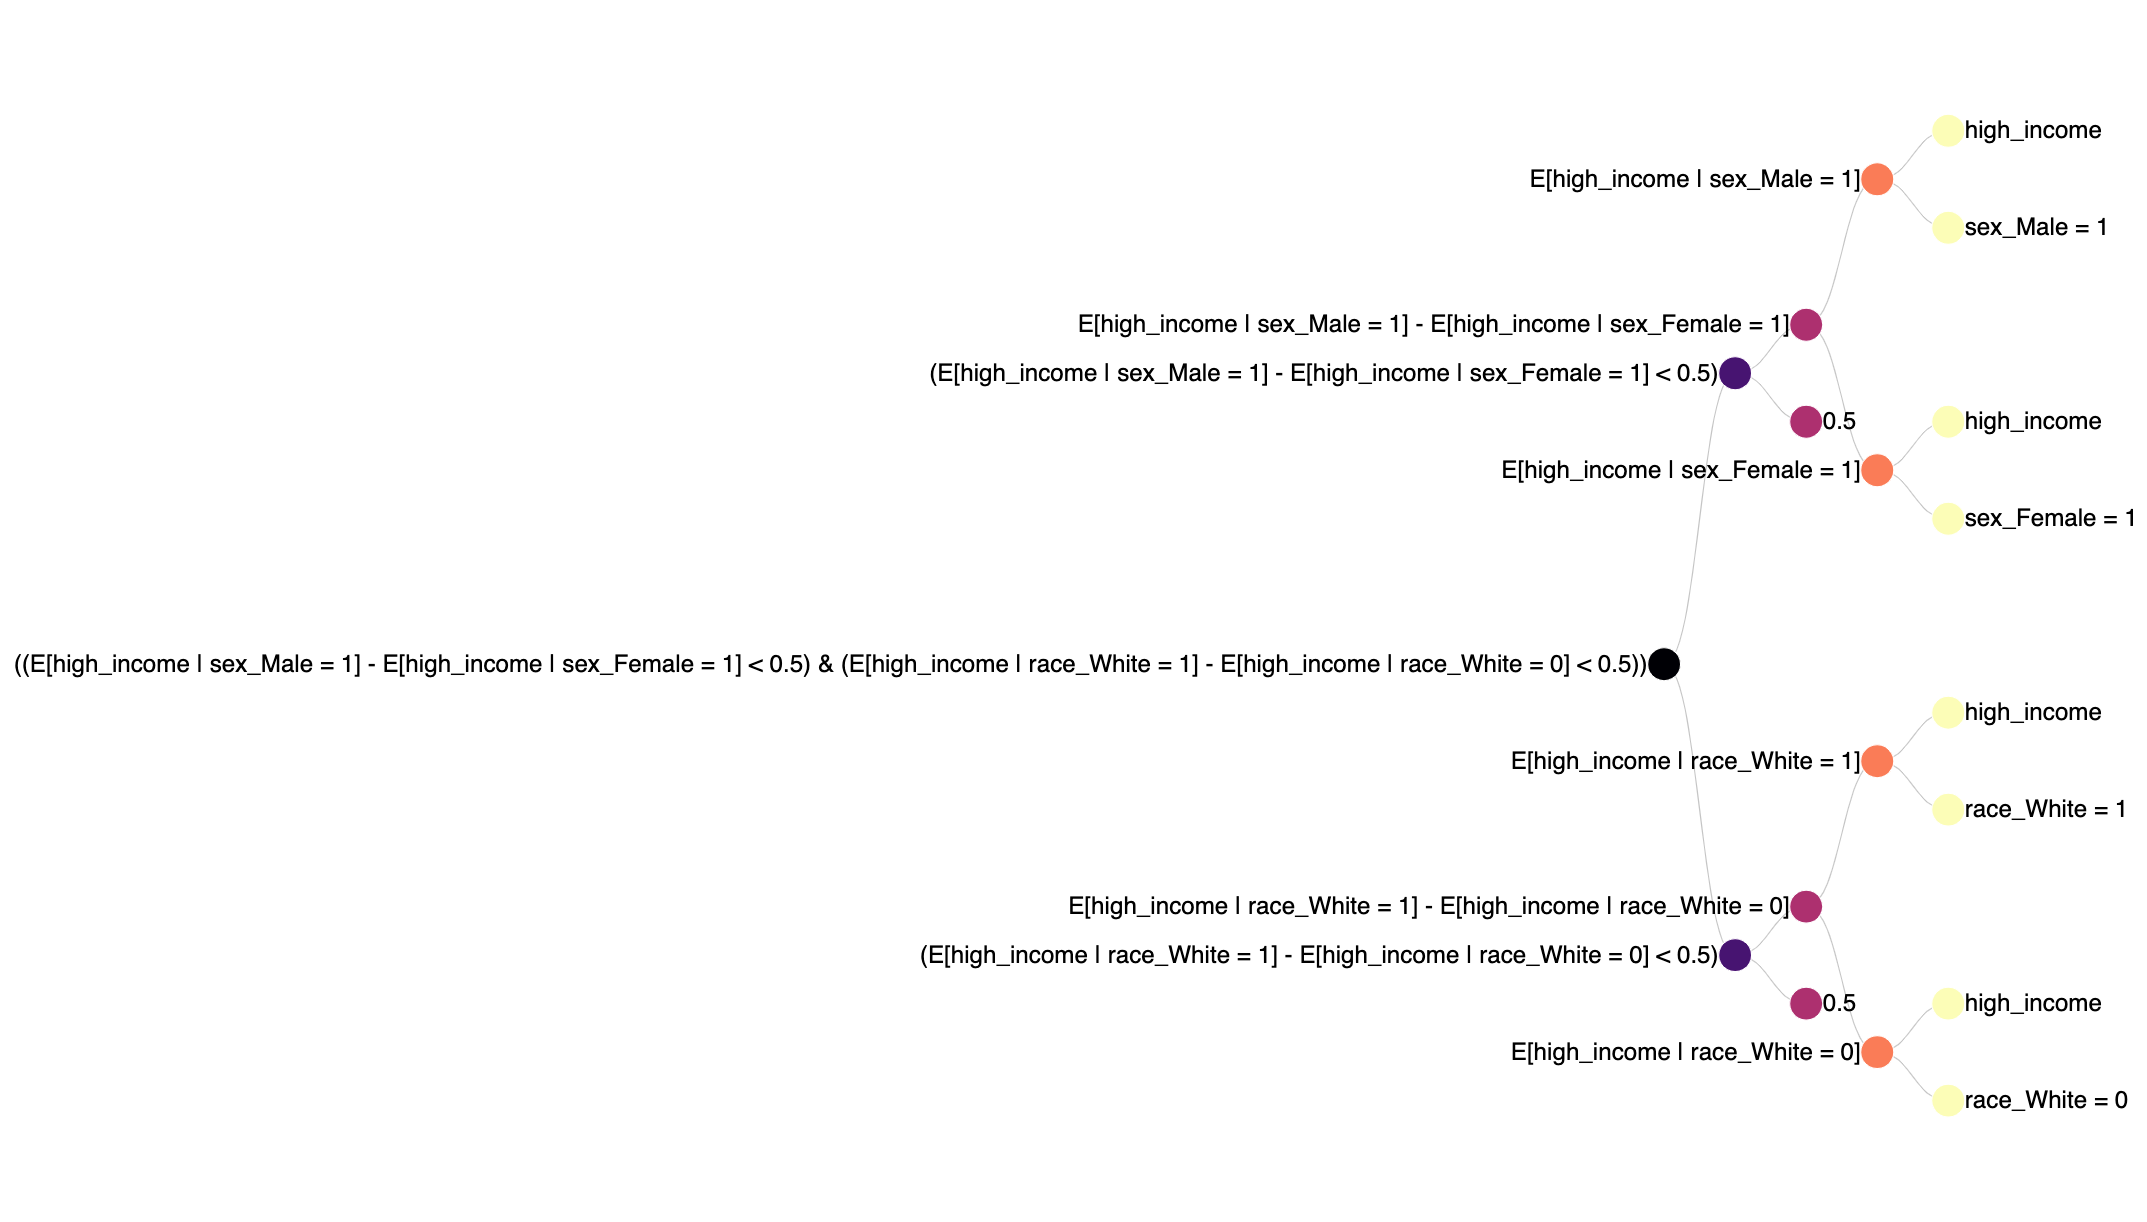
\includegraphics[width=\textwidth, angle=90,alt={Internal representation of parsed tree for a specification.}]{avoir/images/adult-spec-tree-initial.png}
    \caption{Tree corresponding to the initial specification for the Adult Income dataset.}
    \label{fig:impl:adult:initial-spec}
\end{figure}

Using our specification framework as a backend, we built an interactive application for analysis and refinement of specifications provided in our grammar.
Given a user provided machine learning model, dataset, and specification the application simulates a stream of observations to the provided model.
Following the simulation, a visualization is provided that represents the specification as a syntax tree where each node of the tree corresponds to an element of our grammar.
Figure \ref{fig:impl:adult:initial-spec} shows the visualization.

Note that for each observation made by our machine learning model, the specification is evaluated to check for violations.
Each grammar element that makes up the specification is evaluated as well, and thus each grammar element is associated with the value it evaluates to for a given observation.
For specifications \texttt{<spec>}, there is a boolean value associated with each observation, whereas an expectation term, \texttt{<ETerm>}, is associated with a real value.
By selecting one of the nodes in the syntax tree, a user can see a plot of the evaluation values associated with the selected grammar element.
We call these plots evaluation plots and two can be observed at a time 
%(see the plots on the right of figure \ref{fig:casestudy:boston}),
each with shared scales along the horizontal axis which denotes observations over time.
This allows for comparison of multiple grammar elements.
The ability to analyze and compare these evaluation values provides context surrounding specification violations, and assists the user in deciding how to refine a specification.
The case studies in section \ref{sec:casestudy} demonstrate the usefulness of the context provided by these visualizations.

The app for interaction with the backend is built using streamlit. It proceeds in multiple stages,
\begin{enumerate}
    \item First, a user selects a dataset of interest. We built support for four datasets, but our framework is generic enough for any arbitrary csv dataset.
    \item Following this choice, the input variables and output variable for a machine learning model must be specified.
    \item A machine learing model is then selected from a dropdown. We provide support for three models. However, this is for demonstration purposes only - the specification is agnostic to the choice of a machine learning model.
    \item Finally, a specification is input by the user of the app. On the press of a button, the model is trained and then evaluated on the selected dataset. The output monitored by the spec is passed off to the Vega module for further analysis.
\end{enumerate}

\section{AVOIR in Database Setting}

\begin{comment}
\begin{table}
    \centering
    \caption{A summary of the results from the case studies.}
    \label{tab:casestudy:summary}
    \begin{tabular}{ccc}
    \toprule
         Dataset & Setting & Improvement over~\cite{bastani2019probabilistic}  \\
         \midrule
         Adult Income & Database & $10.35\%$ \\
         COMPAS & Materialized View & Interaction\\
         Rate my Profs & ML - BERT & $2.5\%$ \\
         \bottomrule
    \end{tabular}

\end{table}
\end{comment}

In the database literature researchers~\cite{nargesian21tailoring}, have explored an approach to tailoring data integration strategies to ensure that the data set used for analysis has an appropriate representation of relevant (demographic) groups and it meets desired distribution requirements. The authors describe how to acquire such data in an approximate cost-optimal manner for several realistic settings. This work is orthogonal to our work and yet AVOIR can potentially integrate with the authors approach to examine if fairness criteria are being met during the integration process. In other studies on fairness researchers~\cite{yang2018nutritional,asudeh19a,asudeh19b}, have considered the problem of personalized fair ranking functions and discuss approaches to determine if a proposed ranking function satisfies a set of  desired fairness criteria and, if it does not, to suggest modifications that do. AVOIR attempts to solve a  more general purpose problem (not limited to any particular fairness criteria) and is agnostic to the specific model (treats it as a blackbox).  While we have not examined the performance of AVOIR for fair ranking problems, it is something we plan to examine in the future.

To demonstrate how \AVOIRmethodname{} can be integrated within a database system
we use pandas\footnote{https://pandas.pydata.org/} dataframes to simulate the application of \AVOIRmethodname{} in the database setting. 
Specifically, we wrap pandas dataframes with a python `Database' class, and provide a query mechanism to create materialized views.
Queries are provided in the form of python functions that take a dataframe as input and output a corresponding dataframe.
The corresponding view thus generated can be updated with insertion/update/deletion of data.
The specification is added as a decorator inside the refresh function, allowing \AVOIRmethodname{} to track specifications in a database setting.
Note that this tie-in with pandas is only for ease of implementation; the inference engine and optimization can be extended to any database engine.


\end{subappendices}